

\tikzset{every picture/.style={line width=0.75pt}} %set default line width to 0.75pt        

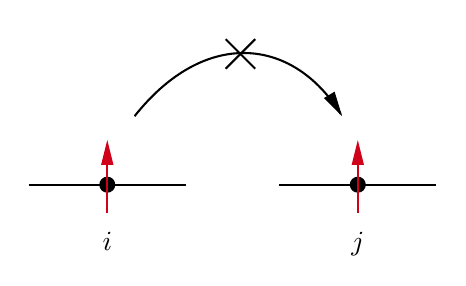
\begin{tikzpicture}[x=0.75pt,y=0.75pt,yscale=-1,xscale=1]
%uncomment if require: \path (0,300); %set diagram left start at 0, and has height of 300

%Straight Lines [id:da7386552192639442] 
\draw    (82,149) -- (157.71,149) ;
%Straight Lines [id:da9226927043104383] 
\draw    (202.71,149) -- (278.41,149) ;
%Straight Lines [id:da04346239197026791] 
\draw    (119.85,149) ;
\draw [shift={(119.85,149)}, rotate = 0] [color={rgb, 255:red, 0; green, 0; blue, 0 }  ][fill={rgb, 255:red, 0; green, 0; blue, 0 }  ][line width=0.75]      (0, 0) circle [x radius= 3.35, y radius= 3.35]   ;
%Straight Lines [id:da49104348516978225] 
\draw    (240.56,149) ;
\draw [shift={(240.56,149)}, rotate = 0] [color={rgb, 255:red, 0; green, 0; blue, 0 }  ][fill={rgb, 255:red, 0; green, 0; blue, 0 }  ][line width=0.75]      (0, 0) circle [x radius= 3.35, y radius= 3.35]   ;
%Straight Lines [id:da7990616031157829] 
\draw [color={rgb, 255:red, 208; green, 2; blue, 27 }  ,draw opacity=1 ]   (119.85,162.5) -- (119.85,129.5) ;
\draw [shift={(119.85,127.5)}, rotate = 450] [fill={rgb, 255:red, 208; green, 2; blue, 27 }  ,fill opacity=1 ][line width=0.08]  [draw opacity=0] (12,-3) -- (0,0) -- (12,3) -- cycle    ;
%Straight Lines [id:da17695895554295893] 
\draw [color={rgb, 255:red, 208; green, 2; blue, 27 }  ,draw opacity=1 ]   (240.56,162.5) -- (240.56,129.5) ;
\draw [shift={(240.56,127.5)}, rotate = 450] [fill={rgb, 255:red, 208; green, 2; blue, 27 }  ,fill opacity=1 ][line width=0.08]  [draw opacity=0] (12,-3) -- (0,0) -- (12,3) -- cycle    ;
%Curve Lines [id:da9848910002402611] 
\draw    (133,116) .. controls (166.37,73.85) and (208.85,77.35) .. (232.3,114.85) ;
\draw [shift={(233,116)}, rotate = 238.87] [fill={rgb, 255:red, 0; green, 0; blue, 0 }  ][line width=0.08]  [draw opacity=0] (12,-3) -- (0,0) -- (12,3) -- cycle    ;
%Straight Lines [id:da5300373220437029] 
\draw    (184,86) ;
\draw [shift={(184,86)}, rotate = 45] [color={rgb, 255:red, 0; green, 0; blue, 0 }  ][line width=0.75]    (-10.06,0) -- (10.06,0)(0,10.06) -- (0,-10.06)   ;

% Text Node
\draw (119.85,170.4) node [anchor=north] [inner sep=0.75pt]    {$\boldsymbol{i}$};
% Text Node
\draw (240.56,170.4) node [anchor=north] [inner sep=0.75pt]    {$\boldsymbol{j}$};


\end{tikzpicture}
